% Generated by code/needham.py -- do not edit by hand.
\definecolor{qocA}{rgb}{0.00,0.45,0.70}
\definecolor{qocB}{rgb}{0.90,0.60,0.00}
\definecolor{qocC}{rgb}{0.00,0.62,0.45}
\definecolor{qocD}{rgb}{0.80,0.40,0.00}
\definecolor{qocE}{rgb}{0.80,0.60,0.70}
\definecolor{qocF}{rgb}{0.35,0.70,0.90}
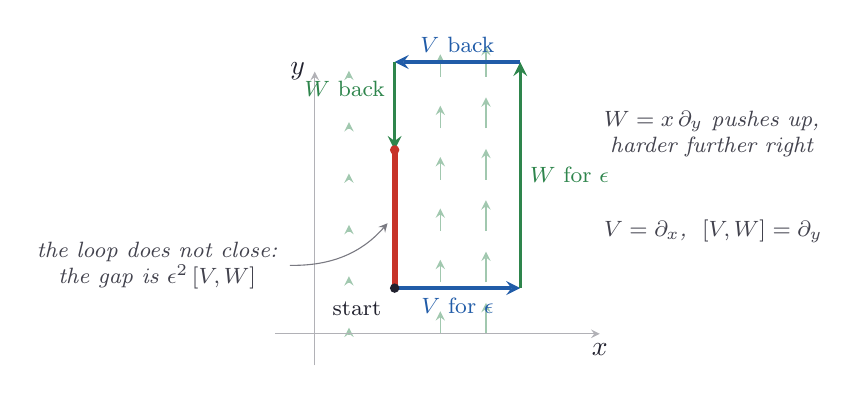
\begin{tikzpicture}[ink/.style={line width=0.9pt, ndInk}, faint/.style={line width=0.4pt, ndInk!35}, dashedink/.style={line width=0.5pt, ndInk!55, dash pattern=on 2.5pt off 2pt}, vec/.style={->, >=stealth, line width=1.2pt}, note/.style={font=\footnotesize\itshape, text=ndInk!85, align=center}, pointer/.style={->, >=stealth, line width=0.4pt, ndInk!60, shorten >=2pt, shorten <=1pt}, dot/.style={circle, fill=ndInk, inner sep=0pt, minimum size=3.4pt}, wash/.style={fill=ndSky, fill opacity=0.55}, every node/.style={text=ndInk}]
\definecolor{ndInk}{rgb}{0.13,0.13,0.18}
\definecolor{ndPaper}{rgb}{0.99,0.96,0.88}
\definecolor{ndSky}{rgb}{0.84,0.91,0.98}
\definecolor{ndRose}{rgb}{0.98,0.86,0.84}
\definecolor{ndBlue}{rgb}{0.13,0.36,0.66}
\definecolor{ndRed}{rgb}{0.78,0.20,0.16}
\definecolor{ndGold}{rgb}{0.88,0.62,0.10}
\definecolor{ndGreen}{rgb}{0.18,0.52,0.30}
\draw[->, >=stealth, line width=0.5pt, ndGreen!45] (0.435,0.000) -- (0.435,0.078);
\draw[->, >=stealth, line width=0.5pt, ndGreen!45] (0.435,0.652) -- (0.435,0.731);
\draw[->, >=stealth, line width=0.5pt, ndGreen!45] (0.435,1.305) -- (0.435,1.383);
\draw[->, >=stealth, line width=0.5pt, ndGreen!45] (0.435,1.958) -- (0.435,2.036);
\draw[->, >=stealth, line width=0.5pt, ndGreen!45] (0.435,2.610) -- (0.435,2.688);
\draw[->, >=stealth, line width=0.5pt, ndGreen!45] (0.435,3.262) -- (0.435,3.341);
\draw[->, >=stealth, line width=0.5pt, ndGreen!45] (1.595,0.000) -- (1.595,0.287);
\draw[->, >=stealth, line width=0.5pt, ndGreen!45] (1.595,0.652) -- (1.595,0.940);
\draw[->, >=stealth, line width=0.5pt, ndGreen!45] (1.595,1.305) -- (1.595,1.592);
\draw[->, >=stealth, line width=0.5pt, ndGreen!45] (1.595,1.958) -- (1.595,2.245);
\draw[->, >=stealth, line width=0.5pt, ndGreen!45] (1.595,2.610) -- (1.595,2.897);
\draw[->, >=stealth, line width=0.5pt, ndGreen!45] (1.595,3.262) -- (1.595,3.550);
\draw[->, >=stealth, line width=0.5pt, ndGreen!45] (2.175,0.000) -- (2.175,0.392);
\draw[->, >=stealth, line width=0.5pt, ndGreen!45] (2.175,0.652) -- (2.175,1.044);
\draw[->, >=stealth, line width=0.5pt, ndGreen!45] (2.175,1.305) -- (2.175,1.696);
\draw[->, >=stealth, line width=0.5pt, ndGreen!45] (2.175,1.958) -- (2.175,2.349);
\draw[->, >=stealth, line width=0.5pt, ndGreen!45] (2.175,2.610) -- (2.175,3.002);
\draw[->, >=stealth, line width=0.5pt, ndGreen!45] (2.175,3.262) -- (2.175,3.654);
\draw[faint, ->, >=stealth] (-0.50,0) -- (3.62,0) node[below] {$x$};
\draw[faint, ->, >=stealth] (0,-0.40) -- (0,3.33) node[left] {$y$};
\draw[vec, ndBlue] (1.015,0.580) -- (2.610,0.580);
\node[below, font=\footnotesize, text=ndBlue] at (1.812,0.580) {$V$ for $\epsilon$};
\draw[vec, ndGreen] (2.610,0.580) -- (2.610,3.451);
\node[right, font=\footnotesize, text=ndGreen] at (2.610,2.016) {$W$ for $\epsilon$};
\draw[vec, ndBlue] (2.610,3.451) -- (1.015,3.451);
\node[above, font=\footnotesize, text=ndBlue] at (1.812,3.451) {$V$ back};
\draw[vec, ndGreen] (1.015,3.451) -- (1.015,2.335);
\node[left, font=\footnotesize, text=ndGreen] at (1.015,3.116) {$W$ back};
\draw[line width=2.2pt, ndRed] (1.015,0.580) -- (1.015,2.335);
\node[dot, label={[font=\footnotesize]below left:start}] at (1.015,0.580) {};
\node[dot, fill=ndRed] at (1.015,2.335) {};
\node[note, anchor=east] (g) at (-0.35,0.87) {the loop does not close:\\the gap is $\epsilon^2\,[V,W]$};
\draw[pointer] (g.east) to[bend right=25] (0.971,1.457);
\node[note, anchor=west] (w) at (3.55,2.54) {$W=x\,\partial_y$ pushes up,\\harder further right};
\node[note, anchor=west] at (3.55,1.30) {$V=\partial_x$, $\;[V,W]=\partial_y$};
\end{tikzpicture}
